\chapter{Campioni chirurgici}

\section{Introduzione ai pezzi chirurgici}

\subsection{La chirurgia elettiva}
Un paziente generalmente va incontro a chirurgia in due situazioni principali. La prima riguarda le chirurgie elettive, ovvero quelle pianificate, in cui c'è una diagnosi o un sospetto diagnostico molto forte che giustifica l’intervento chirurgico. Questo tipo di intervento ha lo scopo di rimuovere un processo patologico, che può essere di natura neoplastica o infiammatoria. Nel caso della chirurgia elettiva, tutto è programmato: il paziente si sottopone all’intervento sulla base di un sospetto diagnostico o di una diagnosi istologica precedente.

\subsection{La chirurgia non elettiva}
La seconda situazione è la chirurgia non elettiva, ovvero un intervento d'urgenza. Questi casi si presentano in varie circostanze, come traumi o, più comunemente in anatomia patologica, perforazioni di visceri. Ad esempio, una perforazione intestinale può derivare dall'ingestione di materiale estraneo o da patologie infiammatorie. In questa categoria, i campioni più frequenti sono quelli derivanti da chirurgie generali, come le appendiciti acute, sebbene oggi si preferisca spesso il trattamento con antibiotici. Altri esempi possono includere perforazioni intestinali o infarti intestinali causati da processi come l'intussuscezione, in cui un segmento dell'intestino si invagina su se stesso, fenomeno associato a masse della parete, soprattutto negli adulti.

\subsection{Finalità del campionamento}
Il campionamento dei pezzi operatori è finalizzato alla formulazione di una diagnosi. Per le patologie neoplastiche, la diagnosi non si limita all'identificazione del tipo di tumore, ma cerca anche di fornire informazioni utili ai vari specialisti che si occupano del paziente oncologico, come oncologi, radioterapisti e chirurghi. Questo approccio è particolarmente importante per identificare i cosiddetti parametri \textit{prognostici} e \textit{predittivi}.\footnote{I parametri \textit{prognostici} forniscono informazioni sul probabile decorso della malattia, indipendentemente dal trattamento. In altre parole, aiutano a prevedere come si comporterà la patologia nel tempo. I parametri \textit{predittivi}, invece, indicano la probabile risposta a un determinato trattamento, aiutando a scegliere la terapia più efficace.} Per quanto riguarda i campioni di chirurgia non elettiva, l'obiettivo è capire il motivo dell'evento acuto o emergente che ha richiesto l'intervento. Anche qui, il fine è quello di formulare una diagnosi precisa. Questo è il motivo per cui il campione viene inviato in anatomia patologica: fornire una risposta che possa guidare la gestione clinica successiva.

\subsection{Apertura del pezzo chirurgico}
I campioni chirurgici, rispetto ai campioni bioptici o di piccole dimensioni, richiedono una cura particolare, soprattutto se il campionamento non viene eseguito tempestivamente dopo il prelievo. In questi casi, il rischio principale è l’autolisi o la sovrainfezione da muffe e batteri presenti sul campione. Per evitare tali complicazioni, si effettua l'apertura del pezzo. Il primo passo, quando il campione arriva in anatomia patologica, consiste nel sezionare il pezzo (se composto da parenchimi) o nell’aprire eventuali cavità, per permettere la penetrazione uniforme della formalina in tutto il campione. La formalina ha la funzione di bloccare tutti i processi biologici, sia quelli interni al campione che quelli derivanti da contaminazioni esterne. Questo procedimento è essenziale per garantire una fissazione omogenea, il che a sua volta assicura una buona immunoreattività del campione, come discusso nel capitolo dedicato alla fissazione.

\subsection{Orientamento del pezzo chirurgico}
Infine, oltre alla sfida del campionamento e della selezione del materiale che sarà processato per ottenere i vetrini, i campioni chirurgici pongono un ulteriore problema: l'orientamento del pezzo anatomico. Ma cosa significa orientare un pezzo chirurgico? Orientare un pezzo chirurgico significa documentare la sua disposizione tridimensionale e identificare con precisione la localizzazione delle strutture anatomiche importanti, come i margini di resezione. Questo passaggio è fondamentale poiché permette di fornire informazioni corrette su eventuali infiltrazioni neoplastiche e su altre caratteristiche rilevanti per la diagnosi e la stadiazione del tumore. Nel prossimo paragrafo vedremo come il campionamento debba tenere conto di questi aspetti per garantire una corretta interpretazione dei risultati da parte del patologo.

\section{Distinzione fra pezzi neoplastici e non neoplastici}

\subsection{Cos'è una neoplasia}
Il termine \textit{neoplasia} deriva dal greco, con il prefisso \textit{neo-} che significa "nuovo" e \textit{plazo} che significa "crescere". Analogamente, in latino, il termine \textit{tumor} si riferisce a un "gonfiore". Entrambi i termini, nel loro significato originario, indicano un processo di crescita anomala che non fa parte della normale anatomia. In epoca moderna, il termine \textit{neoplasia} è usato per indicare un processo cellulare caratterizzato da una proliferazione di cellule anomale che crescono in maniera incontrollata. La neoplasia rappresenta quindi una crescita cellulare fuori dal controllo dei normali meccanismi di omeostasi cellulare.\footnote{In passato, il termine \textit{tumore} era utilizzato per indicare qualsiasi gonfiore anomalo, mentre oggi si riferisce esclusivamente alla proliferazione clonale di cellule mutate, che hanno perso il controllo della crescita. Questo concetto è cruciale per comprendere le malattie neoplastiche.}

\subsection{Caratteristiche delle neoplasie}
Le malattie neoplastiche si presentano, dal punto di vista macroscopico, come masse o crescite anomale all'interno di un tessuto. Per identificare una neoplasia, è necessario avere una profonda conoscenza dell'anatomia normale, poiché l’aspetto macroscopico del campione patologico si confronta sempre con ciò che è considerato normale. Le neoplasie possono manifestarsi in modi diversi: all'interno dei parenchimi come masse che crescono in modo espansivo nelle tre dimensioni, oppure negli organi cavi come una crescita superficiale che si espande progressivamente verso strati più profondi con l'aggressività della neoplasia. Durante il campionamento, è essenziale prestare attenzione anche alle piccole masse, spesso non evidenziate dal chirurgo, poiché in anatomia patologica si ha la responsabilità finale di fornire una diagnosi definitiva.

\subsection{Sierosite}
Le patologie infiammatorie e non neoplastiche si distinguono macroscopicamente da quelle neoplastiche per alcuni aspetti caratteristici. Uno dei segni principali dell'infiammazione è l'opacizzazione delle sierose. Questo fenomeno è spesso osservato in patologie come l'appendicite o le malattie infiammatorie croniche intestinali. Le sierose, come il peritoneo, che normalmente sono lucide, diventano opache e possono essere ricoperte da un induito fibrinoso, ovvero un sottile strato biancastro di fibrina.

\subsection{Infiammazione}
In anatomia patologica, la descrizione macroscopica dell'infiammazione segue i criteri classici di Virchow: \textit{tumor} (gonfiore), \textit{rubor} (rossore), \textit{calor} (calore), \textit{dolor} (dolore) e \textit{functio laesa} (alterazione della funzione). Sebbene non siano tutti apprezzabili macroscopicamente  gonfiore (tumor) e arrossamento (rubor) sono visibili e utilizzati per identificare processi infiammatori. Ad esempio, in un caso di appendicite acuta, l'appendice appare edematosa, rigonfia e arrossata, e può presentare materiale purulento (raccolta di pus). Questo materiale purulento corrisponde, al microscopio, a un infiltrato di neutrofili e tessuto di granulazione. Quando si verificano raccolte più significative di pus, si può parlare di ascessi.

\subsection{Fibrosi e granulomi}
Un altro segno caratteristico di patologie non neoplastiche è la presenza di fibrosi, che distorce l'anatomia normale e può rendere difficile distinguere queste lesioni da masse neoplastiche. Un altro processo che spesso entra in diagnosi differenziale (ovvero si può confondere) con una lesione neoplastica è rappresentato dalle infezioni croniche sostenute da micobatteri o funghi, che possono causare la formazione di granulomi. Queste lesioni possono creare difficoltà diagnostiche, tanto che noduli polmonari non diagnosticati durante biopsie spesso possono essere analizzati in estemporanea dove viene fatta diagnosi di flogosi granulomatosa gigantocellulare con necrosi caseosa (il quadro morfologico della tubercolosi).

\subsection{Campionamento dell'alterazione macroscopica}
In conclusione, i pezzi neoplastici e non neoplastici spesso si distinguono chiaramente dal punto di vista macroscopico. Le neoplasie si presentano come crescite anomale e disorganizzate, spesso di natura espansiva o infiltrativa, mentre le patologie infiammatorie non neoplastiche sono caratterizzate da segni di infiammazione, fibrosi e talvolta raccolte di materiale purulento. La corretta identificazione di questi elementi macroscopici è fondamentale per identificare quali campioni scegliere per la microscopia, e in generale vale la regola in patologia chirurgica che tutte le alterazioni macroscopiche vanno confermate itologicamente.

\section{Campioni neoplastici}

\subsection{Impatto della diagnosi patologica}
La descrizione macroscopica dei campioni neoplastici è cruciale per comprendere la natura e l'estensione del processo patologico. Il referto anatomopatologico rappresenta il documento su cui si basa la gestione futura del paziente oncologico, sia che si tratti di una diagnosi iniziale, sia di una recidiva o di una metastasectomia. Le decisioni cliniche e terapeutiche dipendono strettamente dalle informazioni fornite nel referto.

\subsubsection{Istotipo e Grado}
Il referto anatomopatologico di un pezzo chirurgico è fondamentale nella gestione del paziente oncologico. Esso fornisce una diagnosi definitiva, indicando l’istotipo del tumore e stabilendo il grado di aggressività sulla base di parametri biologici. In particolare, il grado di un tumore descrive quanto esso perde somiglianza rispetto al tessuto di origine.

Ogni tipo di tumore ha il suo sistema di gradazione. Ecco alcuni esempi:
\begin{itemize}
    \item \textbf{Carcinoma spinocellulare:} Il sistema di \textit{Broder} valuta quanto il tumore si differenzia dall'epitelio spinocellulare normale.
    \item \textbf{Carcinoma mammario:} Il grading di \textit{Elston-Ellis} si basa sulla formazione di dotti, il numero di mitosi e il pleomorfismo.
    \item \textbf{Carcinoma della prostata:} Il sistema di \textit{Gleason} valuta l'architettura delle cellule neoplastiche all'interno della prostata.
    \item \textbf{Carcinoma del polmone:} Il carcinoma spinocellulare del polmone segue il grading di Broder, mentre  l'adenocarcinoma polmonare (che oggi rappresenta l'istotipo più frequente) varia in base al sottotipo istologico: i tumori con crescita lepidica sono di grado 1, con crescita acinare o papillare sono di grado 2, mentre quelli con crescita solida o micropapillare sono di grado 3.
\end{itemize}

\begin{figure}[h]
    \centering
    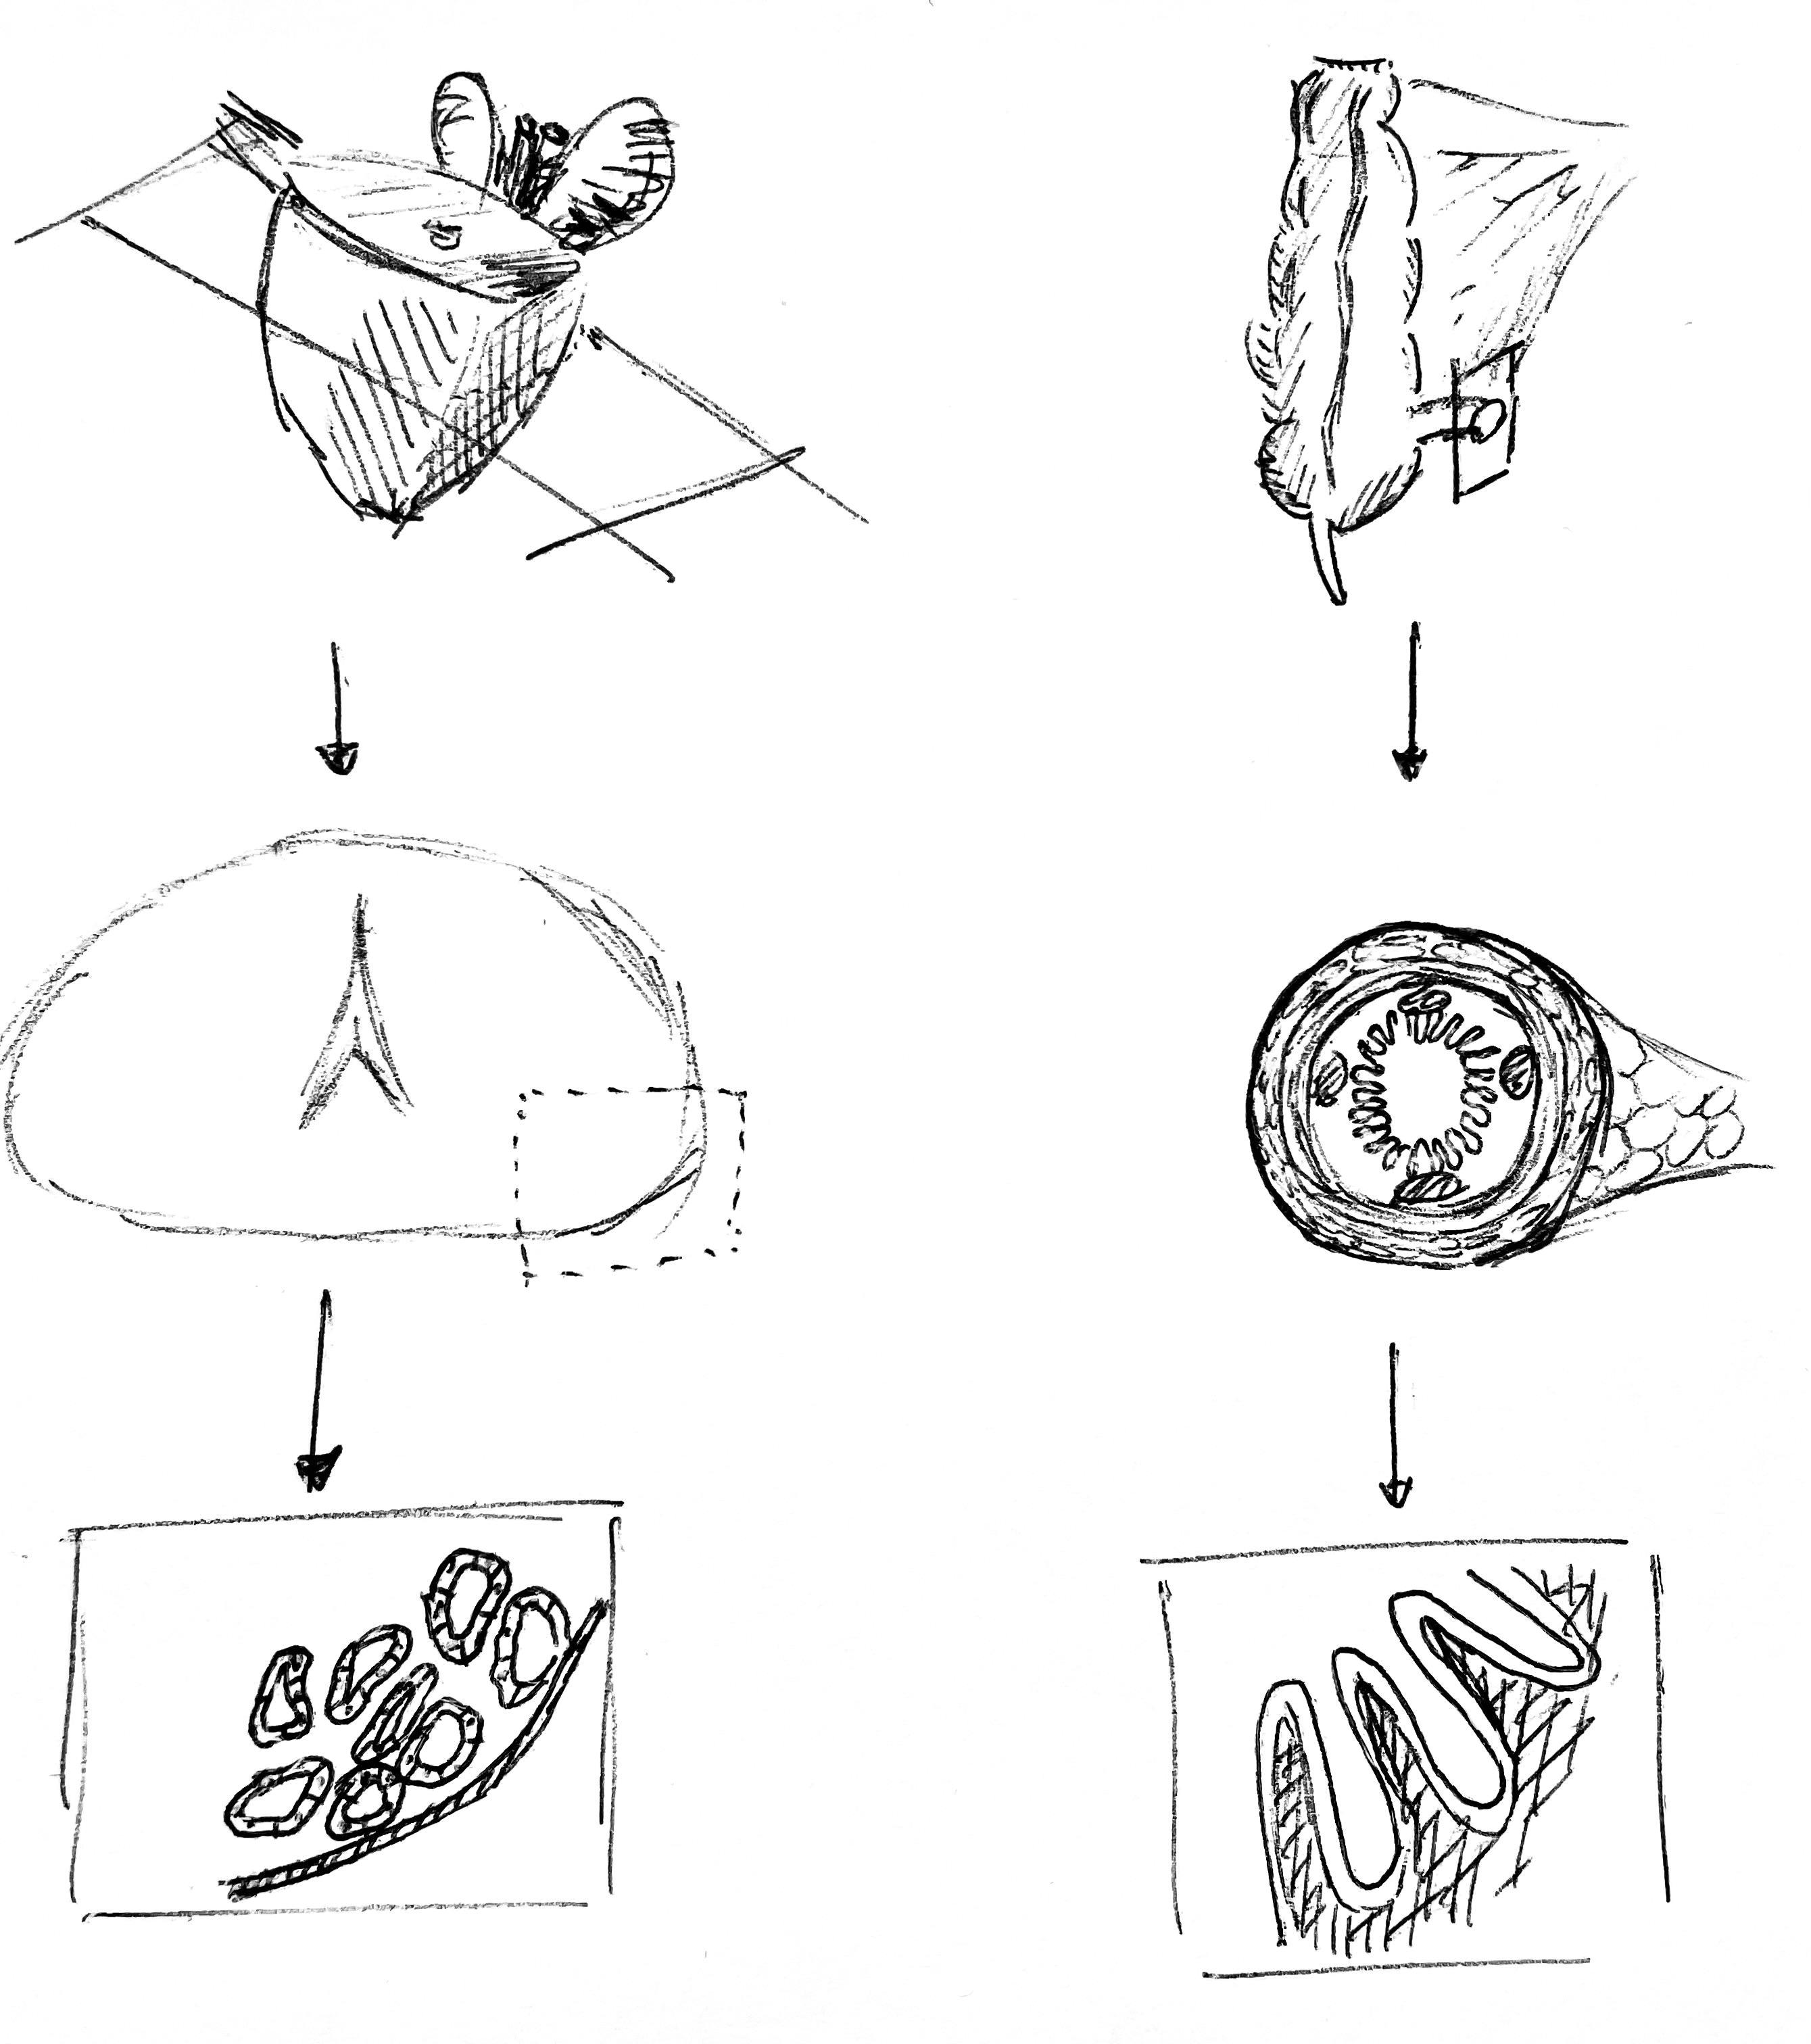
\includegraphics[width=0.85\textwidth]{campionamento_margini}
    \caption{Il campionamento margini}
    \label{fig:campionamento_margini}
\end{figure}

\subsection{Valutazione dei margini chirurgici}
Un elemento fondamentale del referto è la valutazione dei margini chirurgici, che indicano la fine del pezzo anatomico e l'inizio del tessuto sano. I margini possono essere campionati in modi diversi:
\begin{itemize}
    \item \textbf{Margini campionati con inchiostro:} L'inchiostro di china viene applicato per evidenziare il margine anatomico. Se il tumore si trova su questa linea colorata, il margine è considerato positivo (\textit{tumor on ink}).
    \item \textbf{Margini campionati \textit{en face}:} Per organi cavi, il margine viene incluso sul versante che rappresenta il margine anatomico. In questo caso, se vi è tumore sul margine \textit{en face}, il margine è coinvolto.
\end{itemize}

La valutazione dei margini varia a seconda del tipo di tumore. Ad esempio, nel tumore della prostata, la presenza di tumore sulla china indica un margine positivo. In altri casi, una semplice vicinanza del tumore al margine può bastare per stabilire una non radicalità oncologica.

Il sistema di radicalità chirurgica prevede tre livelli:
\begin{itemize}
    \item \textbf{R0:} Radicalità microscopica, ovvero assenza di tumore sui margini.
    \item \textbf{R1:} Positività microscopica del margine.
    \item \textbf{R2:} Positività macroscopica, indicante che il chirurgo non è riuscito a ottenere una radicalità chirurgica completa.
\end{itemize}

\subsection{Stadiazione TNM}
La stadiazione è un altro aspetto critico della valutazione anatomopatologica. Il sistema più utilizzato è il \textit{TNM}, adottato da organizzazioni internazionali come l'UICC (Unione Internazionale Contro il Cancro) e l'AJCC (American Joint Committee on Cancer). Il sistema valuta tre parametri:
\begin{itemize}
    \item \textbf{T:} Dimensioni e estensione del tumore primitivo.
    \item \textbf{N:} Coinvolgimento dei linfonodi (nodes).
    \item \textbf{M:} Presenza di metastasi a distanza.
\end{itemize}

Il patologo è responsabile della stadiazione patologica (\textit{pTNM}), che si differenzia dalla stadiazione clinica (\textit{cTNM}) utilizzata per la diagnosi pre-operatoria. Ogni neoplasia ha un suo sistema di stadiazione TNM. Di seguito, riportiamo una tabella comparativa del sistema TNM per il tumore della mammella e per il tumore del colon:

\begin{table}[h!]
    \centering
    \begin{tabular}{|c|c|c|}
        \hline
        \textbf{Stadio} & \textbf{TNM Mammella} & \textbf{TNM Colon} \\
        \hline
        T1 & Tumore \textless 2 cm & Tumore invade la sottomucosa \\
        \hline
        T2 & Tumore 2-5 cm & Tumore invade la muscolare propria \\
        \hline
        T3 & Tumore \textgreater 5 cm & Tumore invade la sierosa \\
        \hline
        N1 & 1-3 linfonodi coinvolti & 1-3 linfonodi regionali coinvolti \\
        \hline
        N2 & 4-9 linfonodi coinvolti & 4-6 linfonodi regionali coinvolti \\
        \hline
        M1 & Metastasi a distanza presenti & Metastasi a distanza presenti \\
        \hline
    \end{tabular}
    \caption{Confronto tra il sistema TNM della mammella e del colon}
    \label{tab:tnm_comparativo}
\end{table}

\subsection{Importanza del campionamento nella patologie neoplstiche}
Il referto anatomopatologico e la descrizione macroscopica sono essenziali per la diagnosi, la valutazione dei margini e la stadiazione di ogni tumore. Questi elementi determinano il trattamento e la gestione clinica del paziente oncologico, influenzando direttamente il successo terapeutico.

